\section{Resultados}

Con los autómatas definidos así como sus tablas de transición, podemos transcribir los autómatas a un archivo que nuestro programa sea capaz de leer. A continuación veremos 2 quintuplas en operación con nuestro algoritmo y dadas algunas cadenas de entrada, veremos el resultado que producen:

\subsection{AFN-$\epsilon$ 1}

Para el autómata (1) tenemos el siguiente archivo TXT:

\begin{figure}[H]
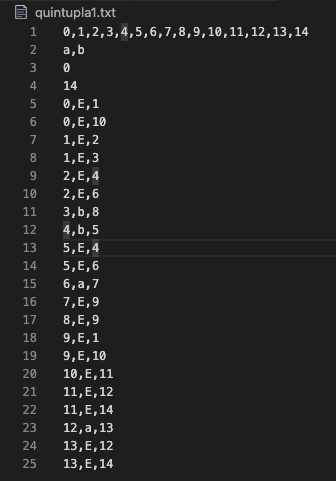
\includegraphics[width = 16.5cm, height = 14cm]{q-1.png}
\centering \linebreak \linebreak {\small Figure 1.0: Quintupla del autómata (1).}
\end{figure} 

Dada la quintupla de la figura 1.0, se genera la siguiente salida en nuestro programa con la cadena \textbf{baa}:

\begin{figure}[H]
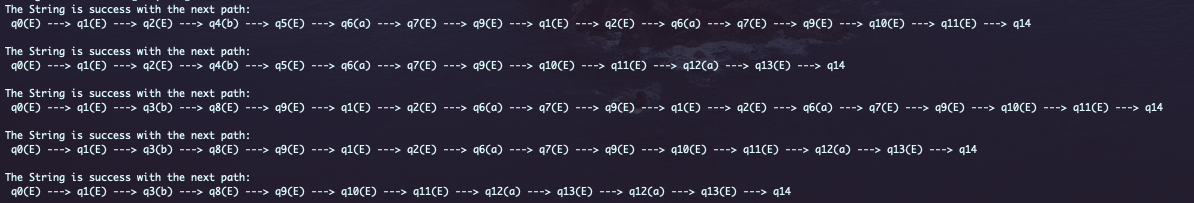
\includegraphics[width = 16.5cm, height = 4cm]{res-aut-1-1.png}
\centering \linebreak \linebreak {\small Figure 1.1: Caminos que la cadena \textbf{baa} puede seguir para llegar a su estado de aceptación.}
\end{figure} 

Dada la quintupla de la figura 1.0, se genera la siguiente salida en nuestro programa con la cadena \textbf{baaa}:

\begin{figure}[H]
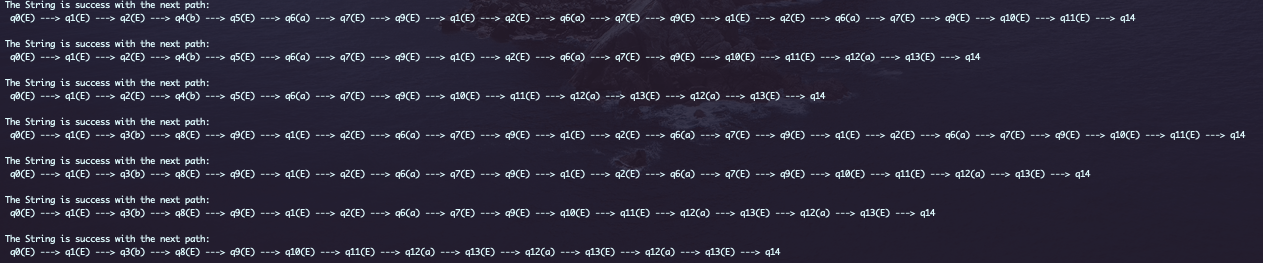
\includegraphics[width = 16.5cm, height = 4cm]{res-aut-1-2.png}
\centering \linebreak \linebreak {\small Figure 1.2: Caminos que la cadena \textbf{baaa} puede seguir para llegar a su estado de aceptación.}
\end{figure}

\subsection{AFN-$\epsilon$ 2}

Para el autómata (2) tenemos el siguiente archivo TXT:

\begin{figure}[H]
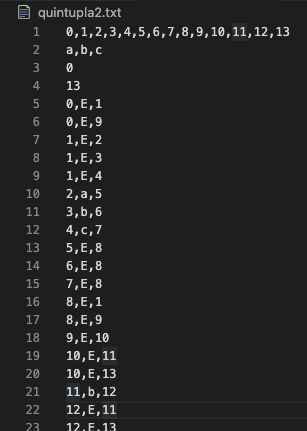
\includegraphics[width = 16.5cm, height = 14cm]{q-2.png}
\centering \linebreak \linebreak {\small Figure 2.0: Quintupla del autómata (2).}
\end{figure} 

Dada la quintupla de la figura 2.0, se genera la siguiente salida en nuestro programa con la cadena \textbf{abb}:

\begin{figure}[H]
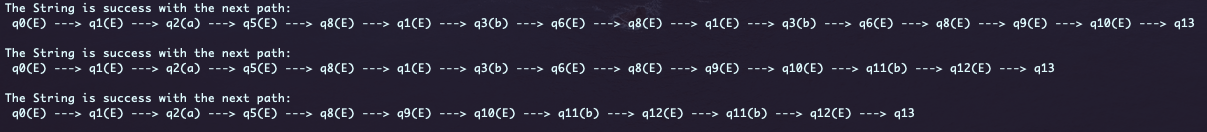
\includegraphics[width = 16.5cm, height = 4cm]{res-aut-2-1.png}
\centering \linebreak \linebreak {\small Figure 2.1: Caminos que la cadena \textbf{abb} puede seguir para llegar a su estado de aceptación.}
\end{figure} 

Dada la quintupla de la figura 2.0, se genera la siguiente salida en nuestro programa con la cadena \textbf{abcbb}:

\begin{figure}[H]
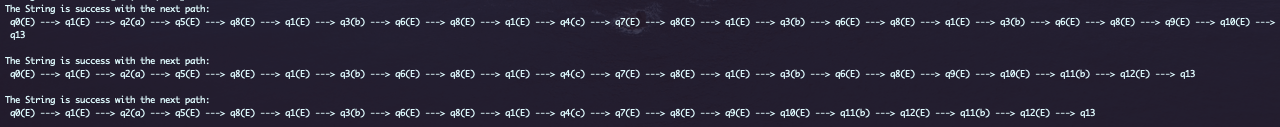
\includegraphics[width = 16.5cm, height = 4cm]{res-aut-2-2.png}
\centering \linebreak \linebreak {\small Figure 2.2: Caminos que la cadena \textbf{abcbb} puede seguir para llegar a su estado de aceptación.}
\end{figure}

\pagebreak